\chapter{Multilagen-PVD}
\label{appendix_multilayer}

\section{Porenbildung bei Unterrelaxation}

Während der Präparation von Kupfer-Nickel-Multilagen-Simulationen haben sich verschiedene defektbehaftete Strukturen gebildet.
Typischerweise deuten Wachstumsdefekte auf geringe Relaxationszeiten, geringe Auftreffenergien oder geringe Temperaturen hin.
Das folgende System wurde bei \SI{500}{\kelvin} mit \SI{5.4}{\electronvolt} Auftreffenergie pro Teilchen für \SI{1.2}{\nano\second} relaxiert.
Die Teilchenenergie liegt mit \SI{5.4}{\electronvolt} vergleichsweise hoch\cite{zhou_atomistic_1998}, wird allerdings vom Thermostat abgedämpft, weshalb die Mobilität des Adatomes verringert und das System unterrelaxiert ist.
Als Resultat bilden sich Poren (Abbildung~\ref{fig:multilayer_surfacefail}), die sich vergleichbar zu den Kupferkratern in Abbildung~\ref{fig:coppercrater} entwickeln, sich aber erst spät wieder schließen.

\begin{figure}[!h]
  \centering
  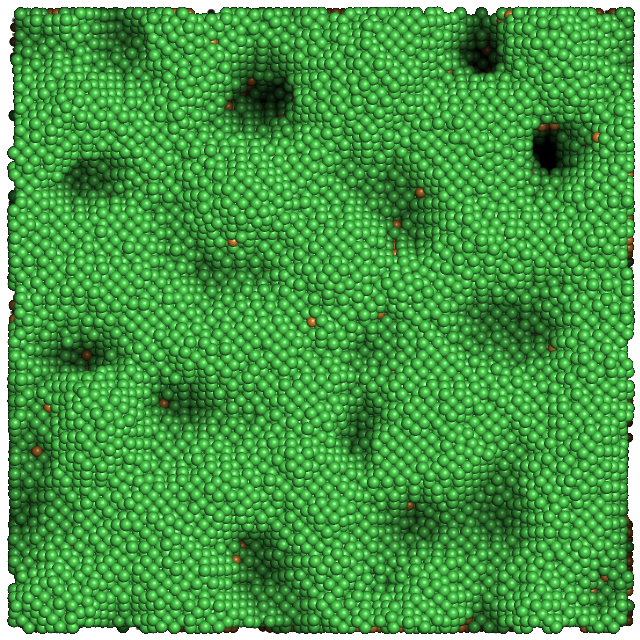
\includegraphics[height=10cm]{CuNi_surface8_noalpha}
  \caption{Oberflächenprofil einer unterrelaxierten CuNi-Oberfläche mit 4 Lagen je \SI{15}{\angstrom}}
  \label{fig:multilayer_surfacefail}
\end{figure}

Abbildung~\ref{fig:multilayer_columnfail} zeigt ein gleichartiges Resultat, das mit denselben Parametern erzeugt wurde.
Hier ist erkennbar, wie sich die gebildeten Poren nach vielen Schichten wieder schließen, wobei zur besseren Veranschaulichung nur ein wenige Nanometer dünnes Profil abgebildet wurde.
Untersuchungen experimentell abgeschiedener Schichten zeigen keine derartigen Fehlstellen\cite{yang_pulsed_1995}, allerdings ist ihre Dicke um einen Faktor von \num{100} höher.
Auch molekulardynamische Untersuchungen\cite{zhou_atomic_2001} fanden keine Bildung von Hohlräumen.
Das Verschwinden der Hohlräume in eigenen Experimenten deutet auf ein Artefakt der Unterrelaxierung hin.

\begin{figure}[!ht]
  \captionsetup[subfigure]{singlelinecheck=false}
  \def\subfigwidth{7cm}
  \begin{subfigure}[t]{\subfigwidth}
    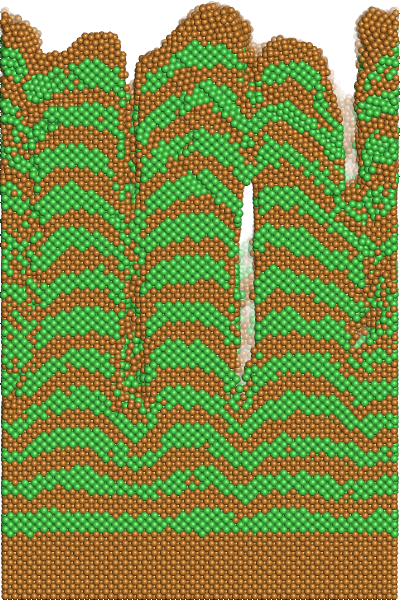
\includegraphics[width=\textwidth]{CuNi_columnfail}
    \subcaption{Dünnes Profil nach 24 Lagen (\SI{180}{\angstrom})}
    \label{fig:multilayer_columnfail}
  \end{subfigure}
  \hfill
  \begin{subfigure}[t]{\subfigwidth}
    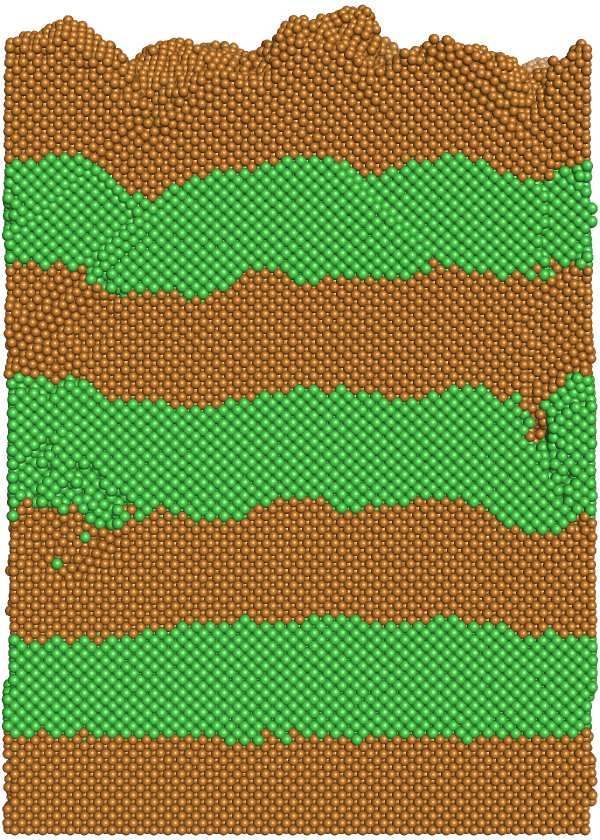
\includegraphics[width=\textwidth]{CuNi_thicklayers}
    \caption{Profil einer Schicht mit 6 Lagen je \SI{6}{\nano\meter}}
    \label{fig:multilayer_thickfail}
  \end{subfigure}
  \caption{Fehlgeschlagene \ce{CuNi}-Abscheidungen während der Parameter-Optimierung}
\end{figure}

\section{Simulationen mit Lagendicken von jeweils \texorpdfstring{\SI{5}{\nano\meter}}{5 nm}}

Ergänzend wurden auch Untersuchungen an Schichten mit Lagendicken begonnen, die sich an technologisch relevanten Werten von mehreren Nanometern orientieren.
Abbildung~\ref{fig:multilayer_thickfail} stellt ein solches System dar, das aber aus Mangel an Rechenzeit für weitere Optimierungszyklen der Simulationsparameter nicht weiter untersucht wurde, weshalb in der Darstellung noch Krater- und Porenbildungen zu beobachten ist, die vermutlich unter Nutzung der optimalen Werte (siehe Kapitel~\ref{multilayer}) eliminiert werden.
